\documentclass[a4paper,parskip,headheight=38pt]{scrartcl} % article or scrartcl
\usepackage[utf8]{inputenc}
\usepackage[T1]{fontenc}
\usepackage{amsmath,amssymb,amsfonts}
\usepackage[%
  automark,
  headsepline                %% Separation line below the header
]{scrlayer-scrpage}
\usepackage[english]{babel}
\usepackage{hyphenat}
\usepackage[hidelinks]{hyperref}
\usepackage[top=1.4in, bottom=1.5in, left=1in, right=1in]{geometry}
\usepackage{lastpage}
\usepackage{csquotes}
\usepackage{microtype}
\usepackage{datetime}

\usepackage[normalem]{ulem}
\usepackage{enumerate}
\usepackage{hyperref}

% \usepackage{multicol}
\usepackage{graphicx}
\usepackage{graphics}
% \usepackage{float}
% \usepackage{caption}

\setkomafont{pagehead}{\normalfont\sffamily\footnotesize}
\addtolength{\headheight}{+6pt}
\lohead{Marlene Böhmer, s9meboeh@stud\ldots, 2547718 \\
	Maximilian Köhl, mail@koehlma.de, 2553525 \\
	Ben Wiederhake, s9bewied@stud\ldots, 2541266}
\rohead{\newline \newline ES16, Set 1, Page {\thepage}/{\pageref*{LastPage}}}

\newtimeformat{mytime}{\twodigit{\THEHOUR}\twodigit{\THEMINUTE}\twodigit{\THESECOND}}
\settimeformat{mytime}
\newdateformat{mydate}{\twodigit{\THEYEAR}\twodigit{\THEMONTH}\twodigit{\THEDAY}}
\cfoot{\tiny\texttt{ID \mydate\today\currenttime}}
\chead{} % Needed because now the \subsections get displayed
\pagestyle{scrheadings}

% \renewcommand{\headrulewidth}{0pt}
% \addtolength{\textheight}{+30mm}
% \addtolength{\textwidth}{+50mm}
% \addtolength{\hoffset}{-7mm}

% \newcommand{\Omicron}{\ensuremath{\mathcal{O}}}
% \newcommand{\omicron}{\ensuremath{o}}
% \newcommand{\set}[1]{\{#1\}}
% \newcommand{\abs}[1]{\lvert #1 \rvert}

\begin{document}

\section*{Problem 1: Simulink}

\subsection*{Part 1: Sketch}

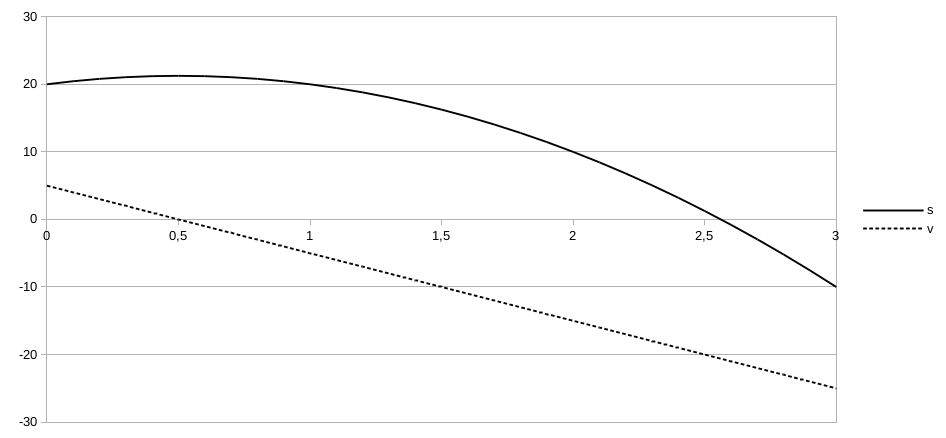
\includegraphics[width=\textwidth]{p1-sketch}

\subsection*{Part 2: Differential equations}

\begin{align*}
    v(0) &= 5 \\
    dv/dt &= -10 \\
    s(0) &= 20 \\
    ds/dt &= v(t)
\end{align*}


\section*{Problem 2: Car Motion on a Slope}

In order to be an equilibrium, the state must have $\dot{x} = 0 \land
\dot{v} = 0$, which implies $v=0$ and (with $v=0$ already applied) $-(m g
\sin \theta) / m = 0$.

One class of equilibria is $g=0, v=0$.  Note that this \enquote{class}
contains infinitely many different states, as we didn't specify $x$.

If one defines $\frac{0}{0} = 0$, then $m=0, v=0$ is another such class.

Since $\theta$ and $F$ are given in the exercise, and can't be changed,
there are no other equilibria.


\section*{Problem 3: Stability of Equilibria}

Reasoning like above:
\begin{align*}
\text{Equilibrium}
&\implies \dot{s}_1 = 0 \land \dot{s}_2 = 0 \\
&\implies 3s_{e1} + 4s_{e2} = 0 \land 2s_{e1} + s_{e2} = 0 \\
&\implies 3s_{e1} + 4(-2s_{e1}) = 0 \land 2s_{e1} + s_{e2} = 0 \\
&\implies s_{e1} = 0 \land s_{e2} = 0
\end{align*}

As there are no other solutions for the equation system, this is the only equilibrium.

Let $\delta > 0$ be arbitrary but fixed, consider the state:
\begin{align*}
s_1(0) := \delta + s_{e1} = \delta && s_2(0) := 0 + s_{e2} = 0
\end{align*}
\begin{align*}
& \dot{s_1}(0) = 3 \delta + 4 \cdot 0 \, \land \, \dot{s_2}(0) = 2 \delta + 0 \\
\overset{\delta > 0}{\implies} & \forall t: \dot{s_1}(t) > 0 \, \land \, \dot{s_2}(t) > 0 \\
\implies & \lim_{t \to \infty} s_1(t) \to \infty \, \land \, \lim_{t \to \infty} s_2(t) \to \infty
\end{align*}
Therefore, it is unstable ($\hat{=}$ not stable and not asymptotically stable).

\section*{Problem 4: Cyclist}

\subsection*{Part 1}

Here is the model we created:

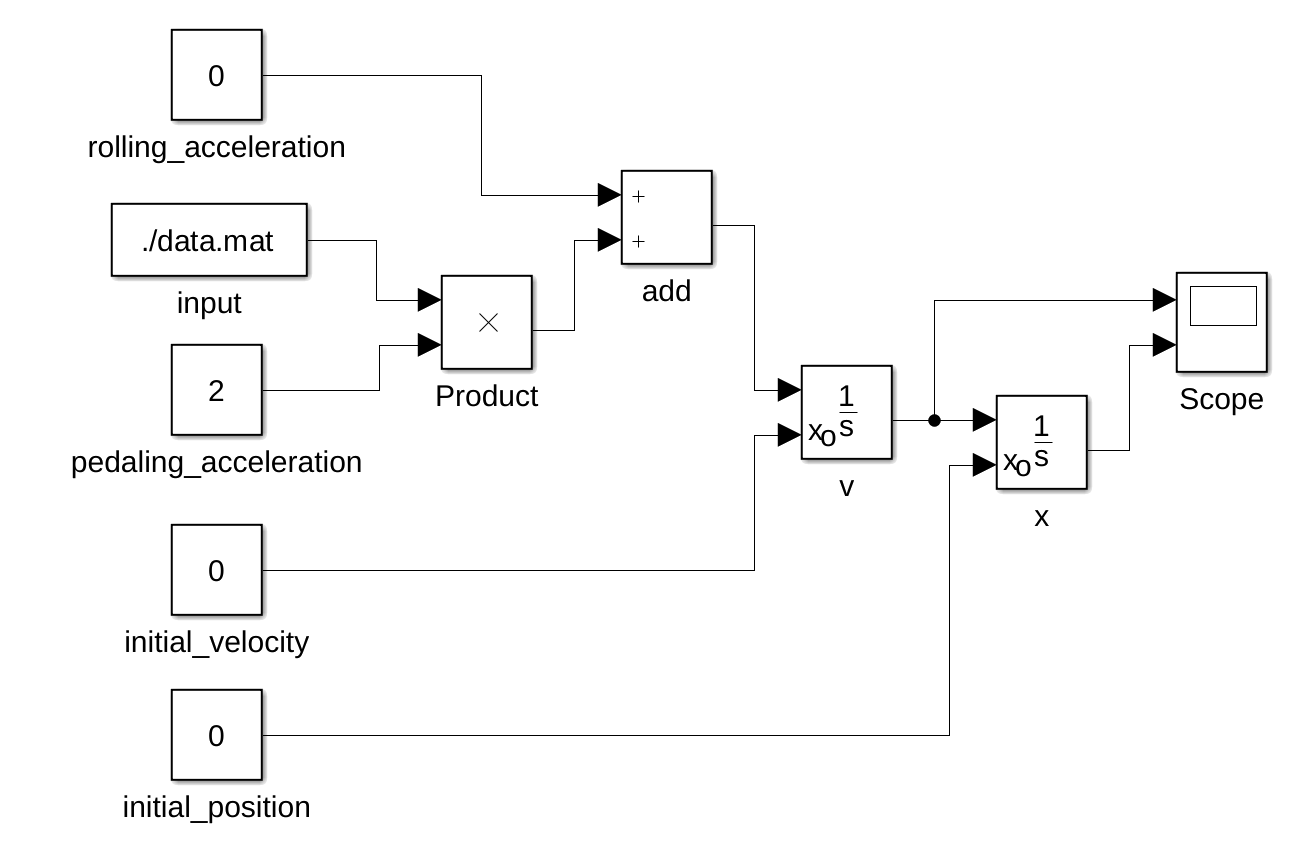
\includegraphics[width=\textwidth]{p4a-proof}

\subsection*{Part 2}

We created an appropriate file and ran a simulation with a sufficiently
small fixed-size step.

\pagebreak{}
Our \texttt{.mat} file can be reproduced like this (in Matlab itself):
%
\vspace{-\baselineskip}\begin{verbatim}
myts = timeseries([]) % matrix-based bags do not support non-linear time
myts = addsample(myts, 'Data', 0, 'Time', 0)
myts = addsample(myts, 'Data', 0, 'Time', 2)
myts = addsample(myts, 'Data', 1, 'Time', 2)
myts = addsample(myts, 'Data', 1, 'Time', 7)
myts = addsample(myts, 'Data', 0, 'Time', 7)
myts = addsample(myts, 'Data', 0, 'Time', 8)
save data -v7.3 myts
\end{verbatim}

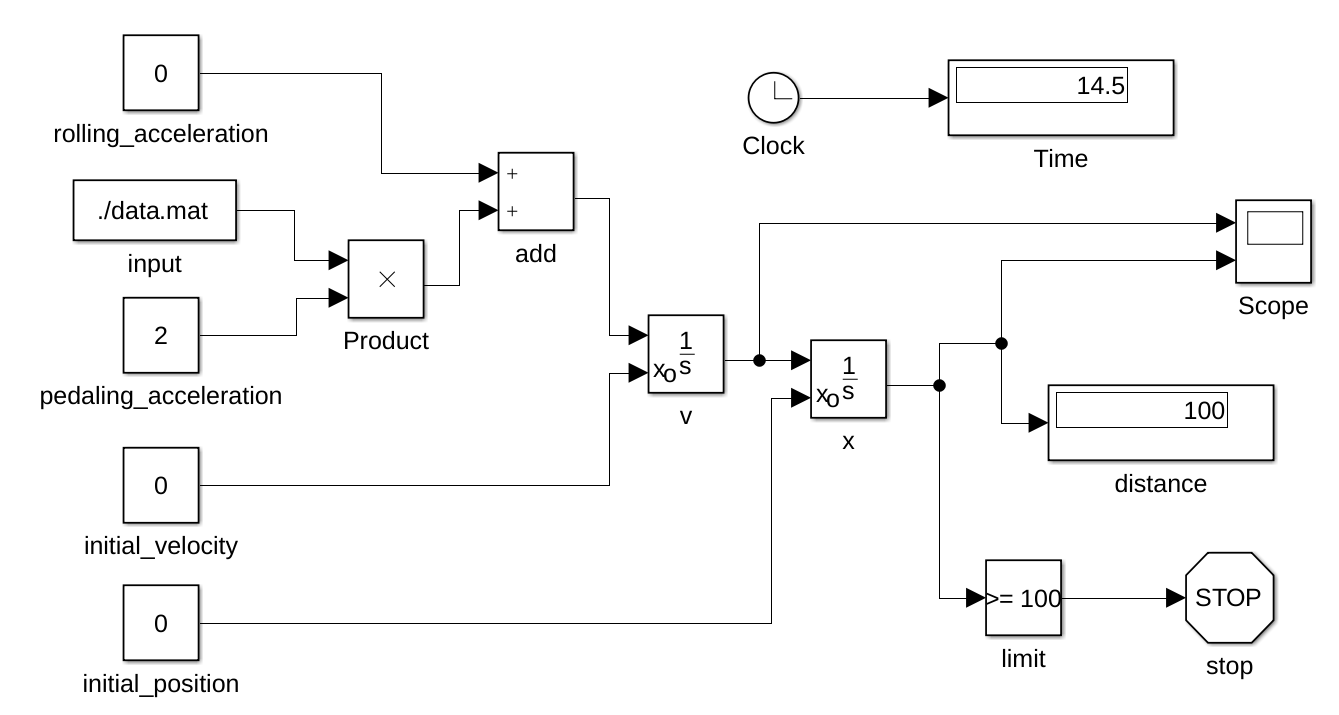
\includegraphics[width=\textwidth]{p4b-proof-small}

The 100m mark seems to be reached at exactly 14.5 seconds with our
starting conditions.


\section*{Problem 5: Oscillator}

\subsection*{Part 1}
\begin{align*}
y_s = \lim_{t \to \infty} y(t) = 0 \\
t_s(0.2) = 103
\end{align*}

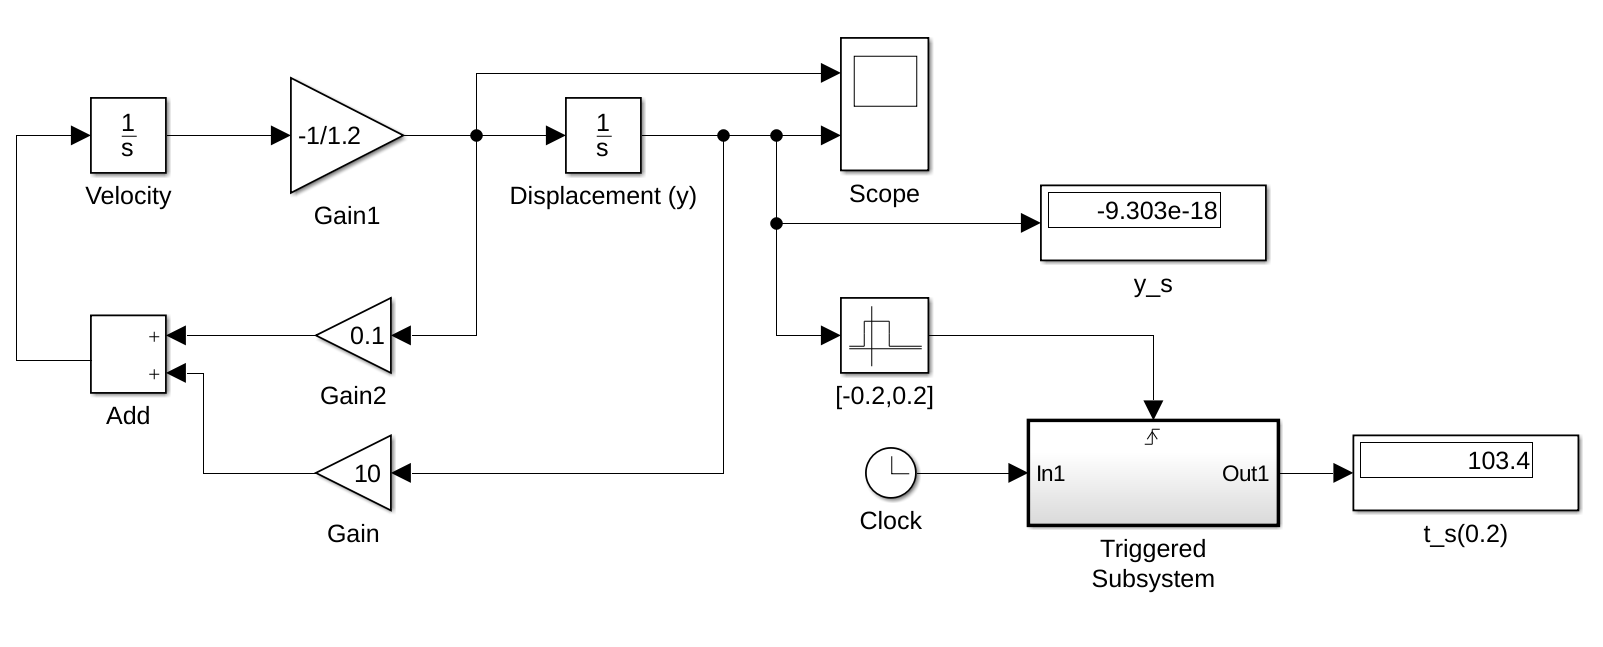
\includegraphics[width=\textwidth]{p5a-proof-small}

\subsection*{Part 2}

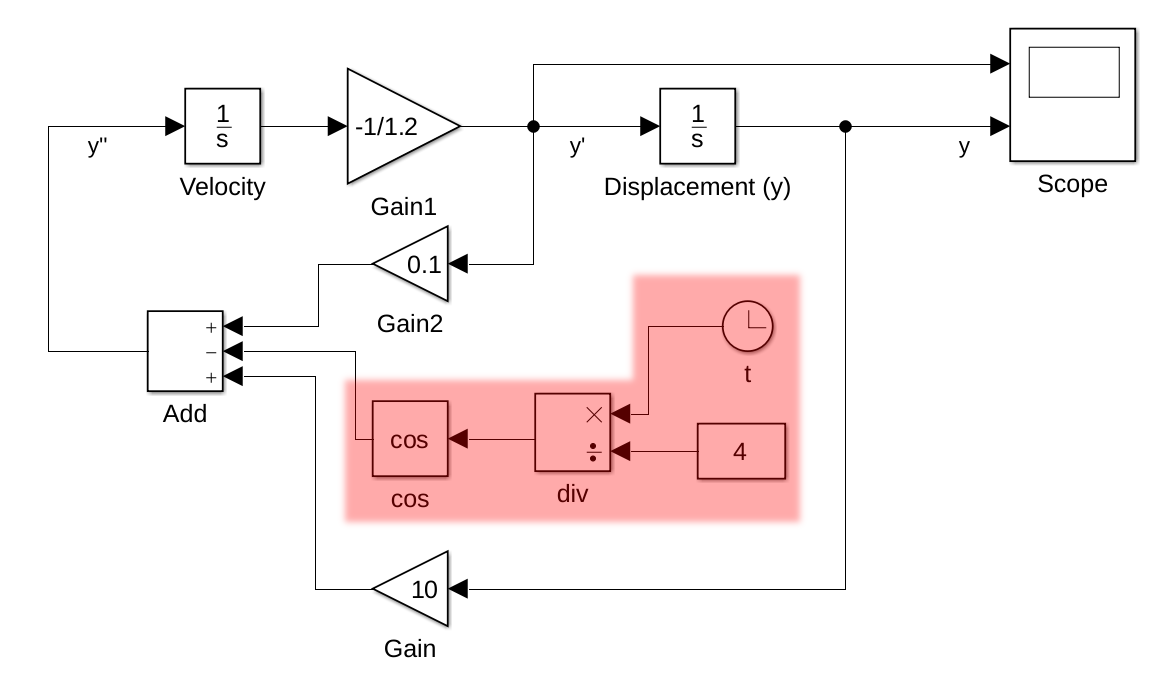
\includegraphics[width=\textwidth]{p5b-model}

We have added the red functional blocks and extended the \emph{Add} block with a new subtraction input.


\section*{Problem 6: Geiger-Müller Counter}

\subsection*{Part 1}

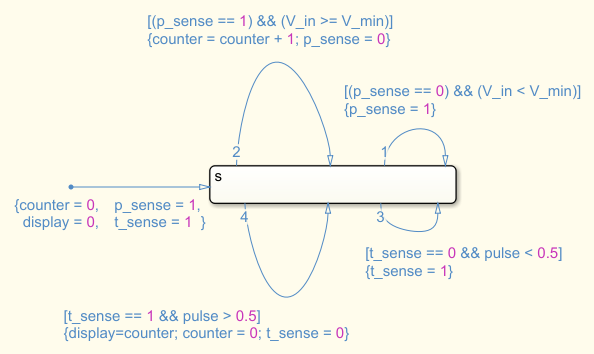
\includegraphics[width=\textwidth]{p6a-model}

Inputs: \texttt{V\_in}, \texttt{V\_min}, \texttt{pulse} \\
Locals: \texttt{counter}, \texttt{p\_sense}, \texttt{t\_sense} \\
Output: \texttt{display}

We couldn't get the \texttt{on every(1,sec)} event to work as intended,
so we use an external pulse generator (\enquote{Simulink/Sources: Pulse
Generator}) that fires every 1 second to trigger the propagation of
\texttt{counter} to \texttt{display}.

The locals \texttt{t\_sense} and \texttt{p\_sense} indicate  sensibility for
another \emph{p}ulse or \emph{t}ime impulse.

The priorities only have an effect when an ionization event
happens exactly on a full second.

 \pagebreak{}
\subsection*{Part 2}

\begin{description}
    \item[How much distortion?] This depends strongly on the variance and
    expected frequency of events.  First of all, notice that the
    counter can never go beyond 10000 events.  Thus, if
    there are \enquote{few} events, the display is reasonably accurate.
    If the display is \enquote{close} to 10000 (on a log
    scale; thus, 1000 already is \enquote{close}), then the
    display is completely inaccurate\footnote{but still not useless: it
    carries the important information \enquote{high radiation, get out
    of here!}}.
        %
    \item[Expected actual number?] Let's say ionization events are
    independent identically distributed (which they seem to be in
    reality).  Let $k$ be the measured number of events.  Then the dead
    time amounted to $k \cdot 0.0001 s$, meaning we actually only
    measured a time span of $1 s - k \cdot 0.0001 s$, which can be used
    to approximate the number of events $n$ in a second by the rule of
    three\footnote{in German: \enquote{Dreisatz}}:
        \[ n \approx k \cdot \frac{1 s}{1 s - k \cdot 0.0001 s}
             = \frac{1}{\frac{1}{k} - 0.0001}\]
    Note that this has the desired properties to stay close to $k$ for
    small values of $k$, and diverge for $k \to 10000$.
\end{description}


\end{document}
